\documentclass[11pt,class=article,float=false,crop=false]{standalone}
\usepackage{Part1_packages}

\begin{document}	

\section{Dynamique des dislocations}

La dynamique des dislocations modélise le déplacement de défauts cristallins dans les matériaux. Les défauts linéiques présents au sein des grains de matériaux cristallins sont appelés Dislocations. Les Dislocations sont à l'origine des déformations plastiques (irréversibles) des composés cristallisés tels que les métaux. Elles évoluent dans la matière et jouent un rôle important dans de nombreux phénomènes qui modifient les propriétés physiques, et notamment leur réponse à l'irradiation qui concerne particulièrement les matériaux du nucléaire.

%Source découverte dislocations : 1934 Orowan, Polanyi, Taylor
%Fundamentals of Materials Science and Engineering

\subsection{Les dislocations}
\label{sec:dislocations}

L'étude des dislocations voit le jour en 1934 avec les publications indépendantes de \textsc{Orowan}, \textsc{Polanyi} et \textsc{Taylor} \todo[inline]{source : dislocations orowan, polanyi et Taylor}. Elles permettent de modéliser la déformation plastique des matériaux. \textit{Introduction to dislocations} par \textsc{Hull} \& \textsc{Bacon} \citebiblio{hull2011introduction} , ainsi que \textit{Theory of Dislocations} par \textsc{Hirth} \& \textsc{Lothe} \citebiblio{hirth1982theory} sont des ouvrages incontournables de la théorie des dislocations.

Dans cette section, nous définirons ce que sont les dislocations, comment leur comportement est modélisé, et quelles sont les conséquences de leur présence sur les propriétés physiques des matériaux.

%https://www.google.fr/url?sa=t&rct=j&q=&esrc=s&source=web&cd=3&ved=0ahUKEwjH7tm7havQAhUJ1RoKHa0oAHkQFggnMAI&url=https%3A%2F%2Fwww.researchgate.net%2Ffile.PostFileLoader.html%3Fid%3D570cf450615e2746b14a8ea3%26assetKey%3DAS%253A350037147176964%25401460466767940&usg=AFQjCNG_3F5KGuiciqHFJUUpKU4t1H5ZHw&sig2=tz0QN9GRCwTVdT_8y7Qq4g&bvm=bv.138493631,d.d2s&cad=rja
%http://deuns.chez.com/sciences/matiere/disloc2.html
%Cours L.Dupuy%
%http://spiralconnect.univ-lyon1.fr/spiral-files/download?mode=inline&data=1874293



\subsubsection{Notions de Mécanique des Matériaux}

La théorie des dislocations est un élément fondamental de la mécanique des matériaux. Avant d'aborder les dislocations, la présentation de quelques éléments de Mécanique des matériaux est nécessaire. Pour un aperçu plus large des concepts de Mécanique des Matériaux, le livre de W.D \textsc{Callister} \citebiblio{callister2013fundamentals} propose un tour d'horizon intéressant du sujet.

\paragraph{Défauts des réseaux cristallins.}

La matière cristallisée est le plus souvent constituée d'une multitude de grains cristallins, à l'image de l'éprouvette de Zirconium de la figure \ref{fig:cristaux:grains}. Dans cette figure, le Microscope Optique à Lumière Polarisée (MOLP) permet de colorer les grains en fonction de leur orientation cristallographique. Chaque grain possède une structure cristalline ou les atomes sont arrangés de manière périodique et régulière. Un motif, appelé maille élémentaire, se répète plusieurs fois pour former un réseau cristallin. Il existe plusieurs types de mailles élémentaires, comme par exemple les structures Cubique Centrée (BCC) et Hexagonale Compacte (HCP) présentées en figure \ref{fig:cristaux:structure}. 

\begin{figure}[H]
	\centering
	\begin{subfigure}[c]{0.39\textwidth}
		\centering
		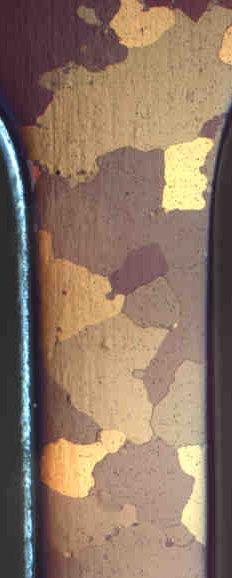
\includegraphics[height=\linewidth]{img/grains-zirconium-molp}
		\caption{Une éprouvette de Zirconium observée au MOLP \citebiblio{lebon2011zr}.}
		\label{fig:cristaux:grains}
	\end{subfigure}
	\begin{subfigure}[c]{0.59\textwidth}
		\centering
		\begin{tabular}{cc}
			\includetikz[2]{img/cubique_centre} &
			\includetikz[1.5]{img/hexagonal_compact} \\
			BCC & HCP
		\end{tabular}
		\caption{Maille élémentaire d'un grain.}
		\label{fig:cristaux:structure}
	\end{subfigure}
	\caption{Structure des matériaux cristallins.}
\end{figure}

Le réseau cristallin peut présenter des défauts qui se manifestent par un mauvais alignement des atomes qui le compose. La figure \ref{fig:defauts} illustre différents exemples de défauts présents dans les cristaux. Un atome en excès (interstitiel) ou en défaut (lacunaire) formera un défaut ponctuel (figure \ref{fig:defauts:ponctuel}), alors que deux cristaux orientés différemment formeront un défaut surfacique, aussi appelé joint de grain (figure \ref{fig:defauts:surfacique}). Les défauts qui nous intéressent particulièrement sont les défauts linéaires, aussi appelés dislocations, qui feront l'objet de la section \ref{sec:dislocations}.

\begin{figure}[H]
	\centering
	\begin{subfigure}[b]{0.49\textwidth}
		\centering
		\includetikz{img/defaut_ponctuel}
		\caption{Défaut ponctuel.}
		\label{fig:defauts:ponctuel}
	\end{subfigure}
	\begin{subfigure}[b]{0.49\textwidth}
		\centering
		\includetikz{img/defaut_planaire}
		\caption{Défaut surfacique.}
		\label{fig:defauts:surfacique}
	\end{subfigure}
	\caption{Défauts dans les cristaux.}
	\label{fig:defauts}
\end{figure}

\paragraph{Phases de déformation.}
De manière générale, les matériaux se déforment en 2 phases, comme l'illustre la courbe contrainte/déformation de la figure \ref{fig:phases_deformation}. 

\begin{figure}[H]
	\centering
	\includetikz{img/stress-strain-phase}
	\caption{Phases de déformation.}
	\label{fig:phases_deformation}
\end{figure}

\newcommand*\circled[1]{\tikz[baseline=(char.base)]{ \node[shape=circle,draw,inner sep=1pt] (char) {#1};} }
\begin{enumerate}[label=\protect\circled{\arabic*}]
	\item \textbf{Elastique} : Une première phase de déformation élastique à lieu à faible déformation et sous faible contrainte. Le matériau est alors déformé de manière réversible tel un ressort. La déformation s'effectue de manière homogène en modifiant l'espace entre les atomes, sans modifier la topologie du réseau cristallin. Le matériau se déforme selon la loi de Hooke qui définit le coefficient élastique $E$.
	
	\item \textbf{Plastique} : Pour des contraintes et des déformations plus élevées une déformation irréversible se produit. La structure du réseau de dislocation est modifiée irrémédiablement par le glissement des dislocations. 
\end{enumerate}
La limite d'élasticité $\sigma _e$ marque la séparation entre les deux phases.



\subsubsection{Les dislocations}

Les dislocations sont les défauts linéaires formés par un demi-plan en excès dans le réseau cristallin. Les déformations plastiques se propagent par le déplacement successif des atomes du réseau, et induit un déplacement des dislocations appelé glissement. La figure \ref{fig:propagation_dislocation} illustre le déplacement d'une dislocation coin ($\bot$) dans un cristal induisant une modification de la topologie du réseau. Le mécanisme de glissement de la dislocation induit un cisaillement : la partie haute du cristal de la figure \ref{fig:propagation_dislocation} glisse latéralement par rapport à la partie basse de celui-ci.

\shorthandoff{:}%
\usetikzlibrary{arrows}
\shorthandon{:}%
\begin{figure}[H]
	\centering
	\begin{subfigure}[b]{0.24\textwidth}
		\centering
		\includetikz[0.8]{img/glissement-cristal-1}
		\label{fig:propagation_dislocation:1}
	\end{subfigure}
	\begin{subfigure}[b]{0.24\textwidth}
		\centering
		\includetikz[0.8]{img/glissement-cristal-2}
		\label{fig:propagation_dislocation:2}
	\end{subfigure}
	\begin{subfigure}[b]{0.24\textwidth}
		\centering
		\includetikz[0.8]{img/glissement-cristal-3}
		\label{fig:propagation_dislocation:3}
	\end{subfigure}
	\begin{subfigure}[b]{0.24\textwidth}
		\centering
		\includetikz[0.8]{img/glissement-cristal-4}
		\label{fig:propagation_dislocation:4}
	\end{subfigure}
	\caption{Déplacement d'une dislocation lors de la déformation plastique.}
	\label{fig:propagation_dislocation}
\end{figure}

Les dislocations sont modélisées par des lignes parcourant le centre des trapèzes que forment les plans successifs, marqué par $\bot$ sur la figure \ref{fig:propagation_dislocation}. On note $\vect{\xi}$ le vecteur directeur de la ligne de dislocation. Par exemple sur la figure \ref{fig:propagation_dislocation}, $\vect{\xi}$ est orthogonal au plan de coupe. 

La déformation du cristal que génère une dislocation est représentée par le vecteur de Burgers $\vect{b}$. Par exemple, dans la figure \ref{fig:propagation_dislocation}, on remarque que la partie haute du réseau se translate vers la droite. La flèche en haut à droite sur chaque figure est le vecteur de Burgers : elle représente le déplacement des atomes au cours du glissement de la dislocation. Ce vecteur à été introduit par \textsc{Burgers} \citebiblio{burgers} \todo[inline]{source : vecteur de Burgers}. Il se définit comme la différence entre le circuit de Volterra dans un cristal parfait et celui autour de la dislocation, comme l'illustre la figure \ref{fig:burgers:volterra}. \footnote{La convention FS/RH issue de \citebiblio{hirth1982theory} est utilisée .}

\begin{figure}[H]
	\centering
	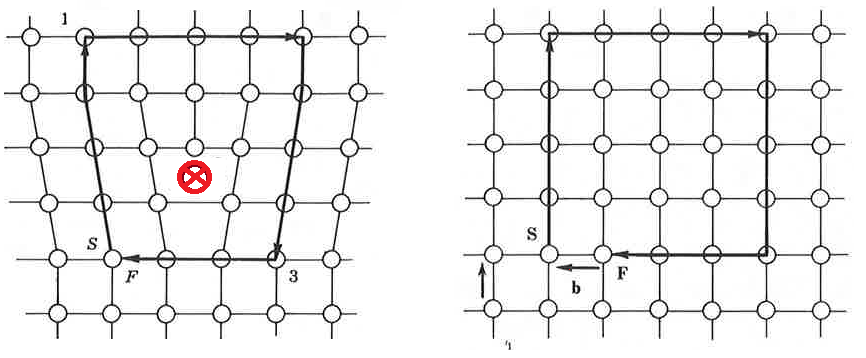
\includegraphics[width=0.6\linewidth]{img/burgers-volterra}
	\caption{Mise en évidence du vecteur de Burgers avec un circuit de Volterra}
	\label{fig:burgers:volterra}
\end{figure} 

La figure \ref{fig:dislocations:schema} représente un réseau simple de dislocations. Le réseau de dislocation peut avoir une géométrie et une topologie complexes lorsque des jonctions sont présentes. Ces dernières se caractérisent par des points où se terminent plusieurs lignes de dislocations ($\bullet$), aussi appelés nœuds physiques.

\begin{figure}[H]
	\centering
	\includetikz[1.5]{img/dislocations}
	\caption{Un réseau de dislocations.}
	\label{fig:dislocations:schema}
\end{figure}

Le vecteur de Burgers à pour particularité de se conserver le long d'une ligne de dislocation, et répond à la loi des nœuds. Pour chaque nœud physique, la somme des vecteur de burgers des dislocations incidentes est nulle. Cette propriété formalisée par l'équation \ref{eq:burgers} est représentée par le triangle en bas de la figure \ref{fig:dislocations:schema}.

\begin{equation}
\sum_{\vect{\xi _i}~entrant} \vect{b_i} = \sum_{\vect{\xi _i}~sortant} \vect{b_i}
\label{eq:burgers}
\end{equation}

\paragraph{}
On distingue deux configurations particulières pour les dislocations selon l'orientation du vecteur de Burgers par rapport à la direction de la ligne.
\begin{itemize}
	\item $\vect{b} \perp \vect{\xi}$ : Lorsque le vecteur de Burgers est orthogonal à la ligne, on parle de dislocation \textit{coin}. Cette situation est par exemple illustrée dans le figure \ref{fig:propagation_dislocation}. Il s'agit d'une configuration très étudiée de par sa simplicité.
	
	\item $\vect{b} \parallel \vect{\xi}$ : Si le vecteur de Burgers est colinéaire à la ligne, on parle de dislocation \textit{vis}.
	
	\item sinon la dislocation est dite \textit{mixte}.
	
\end{itemize}

%%http://www.dwc.knaw.nl/DL/publications/PU00017316.pdf



\subsection{Comportement des Dislocations}
\label{sec:DD:comportement}

\subsubsection{Force de Peach-Koheler}

Les dislocations se déplacent en réponse aux contraintes appliquées sur le cristal. Le mode de déplacement principal des dislocations est le \textit{glissement} où la dislocation se déplace dans son \textit{plan de glissement} contenant les vecteurs $\vect{\xi}$ et $\vect{b}$. Dans certains cas, elles peuvent aussi se déplacer hors de leur plan de glissement lors d'un mécanisme de montée des dislocations.

Dans le cas du glissement, le mouvement des dislocations est régi par la force de Peach-Koheler \citebiblio{peachkoehler1950forces} décrite par la formule \ref{eq:Peach-Koheler}. Cette force par unité de longueur est contenue dans le plan de glissement et orthogonale à la ligne de dislocation. Elle dépend du tenseur de contraintes $\tensor{\sigma}$ dans le matériau.

\begin{equation}
\vect{f}_{PK} = (\tensor{\sigma} \cdot \vect{b}) \times \vect{\xi}
\label{eq:Peach-Koheler}
\end{equation}

\paragraph{}
La contrainte prise en compte pour le calcul de la force résulte des forces externes appliquées au solide, mais aussi des forces internes dues aux interactions entre atomes. Les contraintes externes sont générées par les forces appliquées sur le grain, comme par exemple une compression effectuée par une presse sur le matériau. Les contraintes internes, quand à elles résultent de la déformation du réseau par les défauts qu'il contient, notamment les dislocations.

\begin{equation}
\tensor{\sigma} _{tot} = \tensor{\sigma} _{int} + \tensor{\sigma} _{ext}
\label{eq:contraintes}
\end{equation}

%http://ac.els-cdn.com/0038109894008949/1-s2.0-0038109894008949-main.pdf?_tid=badc76f4-aa4c-11e6-aa73-00000aacb35d&acdnat=1479115901_12bbde1e492a3868cc6c597502a36f38
%Mura Micromechanics of defects in solids - Mura
%http://onlinelibrary.wiley.com/doi/10.1002/pssb.19670200217/pdf

Les dislocation génèrent des contraintes au sein du réseau qui contribuent à $\sigma _{int}$. Les interactions entre dislocations qui en résultent forment la base de la Dynamique des Dislocations.

\subsubsection{Lois de Mobilité}
Selon le type de cristal étudié, on remarque une anisotropie des phénomènes observés. En fonction de l'orientation selon laquelle la contrainte est appliquée, le matériau se déforme plus ou moins facilement. Les dislocations se déplacent préférentiellement dans certains plans (plans denses) selon certains vecteurs de Burgers spécifiques. Il existe donc un nombre restreint de systèmes de glissement (couple plan de glissement + Burgers ) où les dislocations peuvent se déplacer. Par exemple dans les cristaux cubiques face centrés, il existe 12 systèmes de glissements différents dont on retrouve les plans et les Burgers respectivement sur les faces et les arêtes du tétraèdre de Thompson (Fig. \ref{fig:Thompson_tetra}).

\begin{figure}[H]
	\centering
	\includetikz[1.5]{img/tetraedre_thompson}
	\caption{Tétraèdre de Thompson.}
	\label{fig:Thompson_tetra}
\end{figure}

La mobilité des dislocations peut être différente selon le système de glissement. Des études ont pour but de calibrer les lois de mobilités utilisées pour calculer le déplacement des dislocations en fonction de la force appliquée selon le système de glissement \todo[inline]{source : Calibration des mobilités des systèmes de glissement}.

\subsubsection{Formation de jonctions}
Des phénomènes locaux peuvent se produire lorsque deux lignes de dislocation entrent en contact. Dans certains cas, il peut y avoir formation de jonctions : les lignes de dislocation fusionnent. Les jonctions peuvent se former à partir de la collision entre deux dislocation ou plus. Par exemple on observe sur la figure \ref{fig:jonctions:plan} deux dislocations dans le même plan formant une jonction. Les cas ou plusieurs dislocation entrent en contact peuvent mener à des situations plus complexes comme dans la figure \ref{fig:jonctions:3D};

\begin{figure}[H]
 	\centering
 	\begin{subfigure}[t]{0.49\textwidth}
 		\centering
 		\raisebox{-0.5\height}{\includetikz[0.75]{img/jonction-plan}}
 		\caption{Une jonction planaire entre deux dislocations.}
 		\label{fig:jonctions:plan}
 	\end{subfigure}
 	\begin{subfigure}[t]{0.49\textwidth}
 		\centering
 		\raisebox{-0.5\height}{\includetikz[0.75]{img/junction-zip}}
 		\caption{Une multi-jonction formant une source de Frank-Read \citebiblio{bulatov2006nature}.}
 		\label{fig:jonctions:3D}
 	\end{subfigure}	
 	\label{fig:jonctions}
 	\caption{Formation de jonctions.}
\end{figure}

De nombreuses études s'intéressent aux phénomènes de formation de jonctions et à leur impact, notamment sur les phénomènes d'écrouissage \citebiblio{bulatov2006nature,madec2002junctions}. Nous verrons plus tard que la gestion des phénomènes locaux comme la formation de jonctions est un enjeu majeur afin de simuler de manière fidèle la Dynamique des Dislocations.

\subsection{Rôle dans le comportement des matériaux}
\label{sec:DD:effets}

Ormis le mécanisme de déformation plastique présenté plus haut, la théorie des dislocation permet de mieux comprendre et modéliser certains phénomènes liés aux propriétés des matériaux. Nous évoquerons ici les phénomènes d'écrouissage et de durcissement par irradiation.

\subsubsection{Écrouissage}

Lorsque un matériau est déformé plastiquement, ses propriétés physiques sont durablement modifiées. Par exemple, la limite de déformation plastique est repoussée (durcissement) comme le montre la figure \ref{fig:ecrouissage}. Dans cette figure, une première traction \circled{1}est effectuée sur le matériau au delà de la limite élastique. Une fois le matériau définitivement déformé, la contrainte est relaxée et l'échantillon reprend une position au repos légèrement plus allongée. Lorsqu'une contrainte est de nouveau appliquée \circled{2}, on remarque que la limite élastique est plus grande et correspond à la contrainte maximale de la première traction.

\begin{figure}[H]
	\centering
	\includetikz[1]{img/ecrouissage}
	\caption{Écrouissage.}
	\label{fig:ecrouissage}
\end{figure}

Ce phénomène est directement lié à la densification du réseau de dislocation lors d'une déformation plastique. Les jonctions qui forment un obstacle au déplacement des dislocation sont plus nombreuses, et la déformation plastique apparaît donc pour des contraintes plus élevées.

La relation de Taylor \todo[inline]{source : relation de Taylor} donne la limite élastique en fonction de la densité de dislocations:

\begin{equation}
\sigma _e (\rho) = \sigma _i + \alpha \mu b \sqrt{\rho}
\end{equation}
\begin{itemize}
	\item $\sigma _e$ la limite élastique du matériau;
	\item $\sigma _i$ la limite élastique du cristal parfait;
	\item $\alpha$ une constante;
	\item $\mu$ le module de cisaillement du matériau;
	\item b le vecteur de burgers;
	\item $\rho$ la densité de dislocations (en $m/m^3$);
\end{itemize}

L'étude des mécanismes de écrouissage est la principale motivation du développement du code ParaDis \citebiblio{bulatov2006nature}. Nous verrons en section \ref{sec:resultats ddd} ce que la Dynamique des Dislocations a apporté à la compréhension de ce mécanisme.

\subsubsection{Irradiation}

\paragraph{Effets de l'irradiation}

Les effets de l'irradiation sur les matériaux sont multiples, comme le durcissement, la fragilisation ou encore le fluage. 
\begin{itemize}
	\item le durcissement augmente la limite d'élasticité;
	\item la fragilisation réduit la déformation maximale avant rupture
	\item le fluage est une déformation du matériau malgré que la contrainte ne varie pas.
\end{itemize}

La courbe \ref{fig:irradiation-stress-strain} présente une comparaison des courbes contrainte/déformation d'un matériau irradié et non irradié.

\begin{figure}[H]
	\centering
	\includetikz{img/irradiation-stress-strain}
	\caption[Courbe contrainte déformation du fer selon la dose de radiation]{Courbe contrainte déformation selon la dose de radiation}
	\label{fig:irradiation-stress-strain}
\end{figure}



\paragraph{Boucles d'irradiation}

Lors de l'irradiation, la structure des cristaux est modifiée, et les défauts qui se forment peuvent être modélisées par des boucles d'irradiation. Ces boucles d'irradiation que l'on peut voir dans la figure \ref{fig:boucles_irradiation} forment un obstacle à la progression des dislocations, générant alors des phénomènes de durcissement.

\begin{figure}[H]
	\centering
	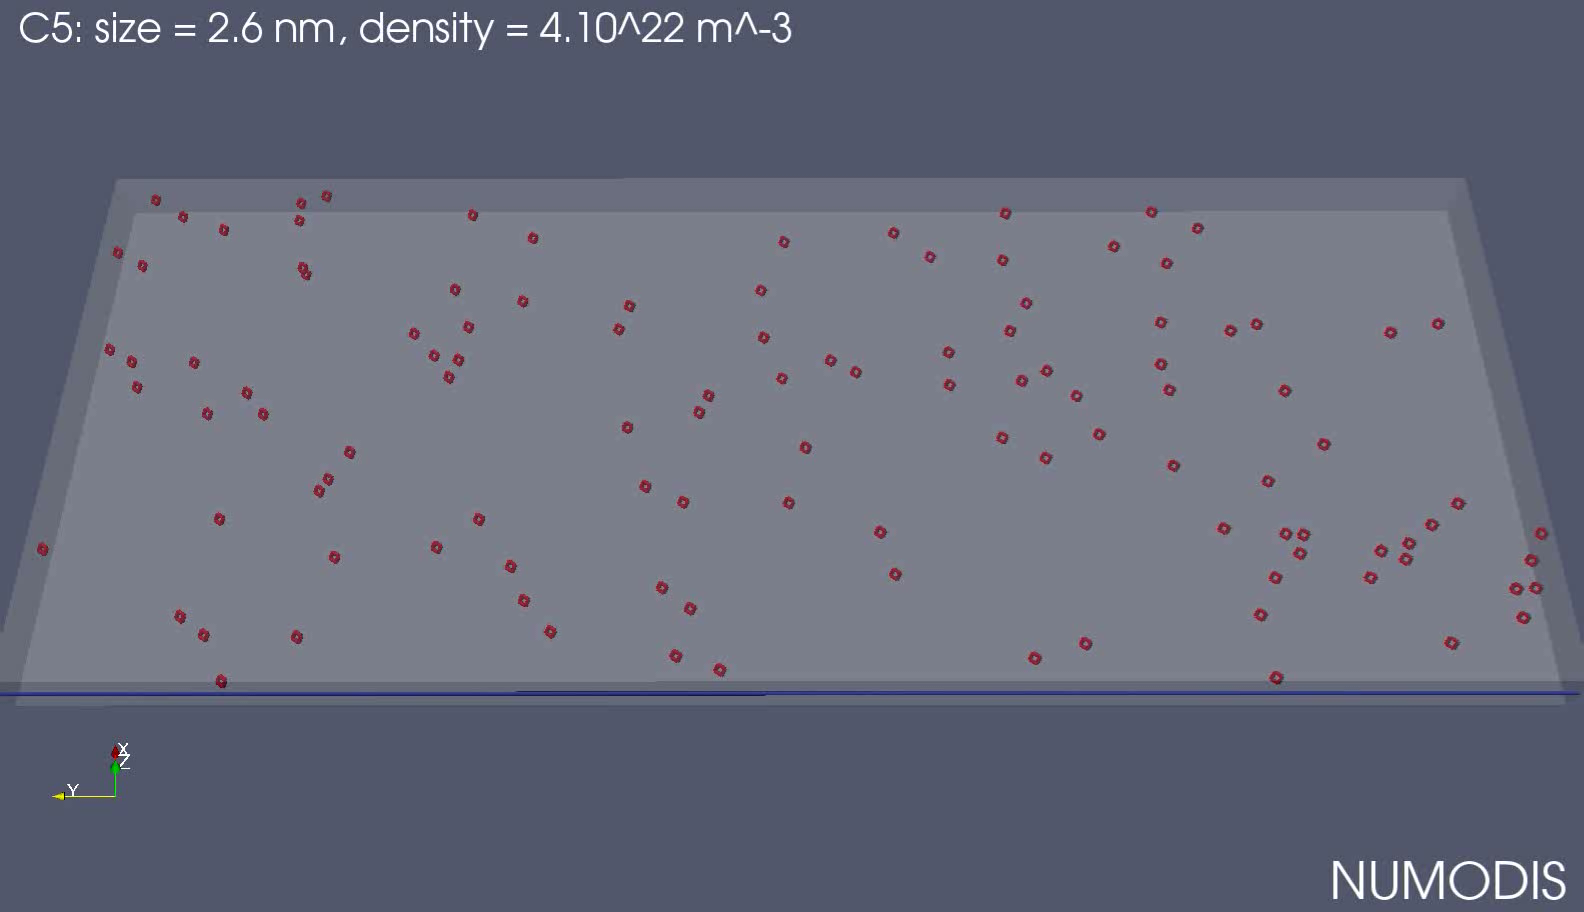
\includegraphics[height=0.3\textheight]{img/boucles-irradiation}
	\caption[Déplacement d'une ligne de dislocation dans un champ de boucles d'irradiation]{Déplacement d'une ligne de dislocation dans un champ de boucles d'irradiation \citebiblio{shi2014these}.}
	\label{fig:boucles_irradiation}
\end{figure}

\paragraph{}

C'est la modélisation des ces phénomènes liés à l'irradiation qui a motivé le développement de NumoDis/OptiDis \citebiblio{optidis}. Nous verrons en partie \ref{sec:resultats ddd} quelles sont les études menées à ce sujet.



\subsection{La DD dans un contexte multi-échelle}
\label{sec:multiscale_modeling}

La modélisation multi-échelle vise à comprendre le comportement des matériaux en analysant les mécanismes physiques élémentaires à plusieurs échelles. Elle consiste à remonter aux principes les plus élémentaires des interactions au sein de la matière - \textit{ab initio} - , pour ensuite modéliser à des échelles de plus en plus grande son comportement. Différents phénomènes sont modélisés de l'échelle des particules élémentaires jusqu’à la structure complexe d'une centrale. La figure \ref{fig:multiscale} montre différentes théories et échelles utilisées dans la Modélisation Multi-échelle des Matériaux. La modélisation à chaque étape se base sur les résultats obtenus aux échelles inférieures, et sert à son tour de base pour la modélisation des échelles supérieures.

\begin{figure}[H]
	\centering
	\includetikz{img/multiscale_modeling}
	\caption{Modélisation Multi-échelle des Matériaux}
	\label{fig:multiscale}
\end{figure}

\paragraph{Dynamique moléculaire}

La dynamique moléculaire simule indépendamment le comportement de chaque atome du matériau considéré. Elle modélise de manière très précise le comportement des matériaux, mais est très coûteuse en temps de calcul. Il est possible d'en extraire des informations sur le comportement des dislocations à petite échelle pour calibrer les modèles de Dynamique des dislocations.

\paragraph{Éléments finis, FFT}

Pour des échelles plus grandes, des simulations utilisant les éléments finis ou la FFT sont utilisées comme le code AMITEX-FFTP \citebiblio{amitex-fftp}. Les échelles considérées permettent leur utilisation dans l'industrie, mais nécessite une calibration, notamment par la Dynamique des Dislocations.

\subsubsection{Validation}

\paragraph{Comparaison expérimentales}

Les résultats de dynamique des dislocations peuvent être validés par l'expérience en comparant les grandeurs macroscopiques, ou grâce à la l'observation in situ du déplacement des dislocations.
Par exemple, dans sa thèse \citebiblio{shi2014these}, X. \textsc{Shi} propose une validation en utilisant comme grandeur macroscopique la contrainte d'écoulement d'une dislocation dans un champs de boucles d'irradiation (fig. \ref{fig:boucles_irradiation}).
Des comparaisons à des observation MET in-situ ont aussi été proposées par J. \textsc{Drouet} \citebiblio{drouet2016comparaison}, comme nous pouvons l'observer dans la figure \ref{fig:comparaison-met-insitu}

\begin{figure}[H]
	\begin{subfigure}[b]{0.5\textwidth}
		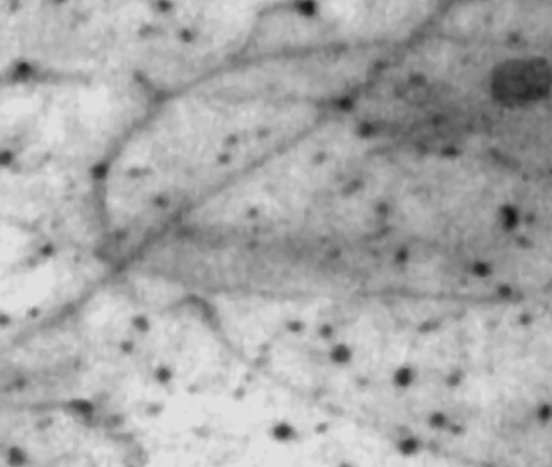
\includegraphics[width=\textwidth]{img/julie-met}
		\caption{Microscope Électronique en Transmission.}
	\end{subfigure}
	\begin{subfigure}[b]{0.49\textwidth}
		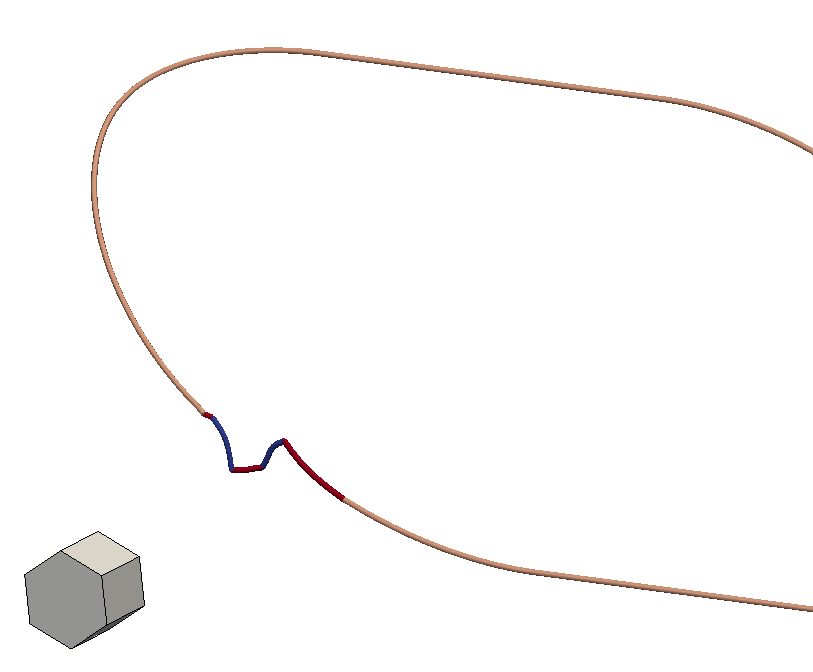
\includegraphics[width=\textwidth]{img/julie-dd}
		\caption{Simulation de Dynamique des Dislocations.}
	\end{subfigure}
	\caption[Validation par des observations MET]{Validation par des observations MET in-situ \citebiblio{drouet2016comparaison}.}
	\label{fig:comparaison-met-insitu}
\end{figure}

De nouvelles techniques permettent maintenant d'observer les dislocations avec la tomographie 3D depuis des images de Microscope Électronique en Transmission \citebiblio{tomo3d} \todo[inline]{Source tomographie 3D}. La figure \ref{fig:tomo3d} donne un exemple ce ce qu'il est possible d'observer avec cette technique.

\begin{figure}[H]
	\centering
	\missingfigure[figwidth=0.49\linewidth]{Tomographie 3D Dislocations}
	\caption[Reconstruction du réseau de dislocations en 3D à partir d'images MET]{Reconstruction du réseau de dislocations en 3D à partir d'images MET\citebiblio{tomo3d}.}
	\label{fig:tomo3d}
\end{figure}


\paragraph{Dynamique Moléculaire}

La Dynamique Moléculaire apporte une base de validation aux simulations de Dynamique des Dislocations. La figure \ref{fig:comparaison_md} illustre les comparaisons DD/MD menées par XJ Shi \citebiblio{shi2015comparaison} montrent une adéquation entre les deux méthodes de simulation.

\begin{figure}[H]
	\centering
	\begin{subfigure}[b]{0.49\textwidth}
		\centering
		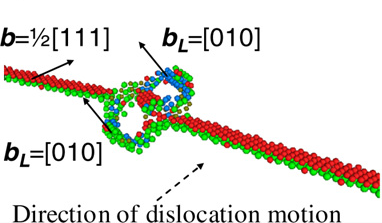
\includegraphics[height=0.15\textheight]{img/comparaison-xshi-md}
		\caption[Dynamique Moléculaire]{Dynamique Moléculaire \citebiblio{terentyev2008simulation}.}
	\end{subfigure}
	\begin{subfigure}[b]{0.49\textwidth}
		\centering
		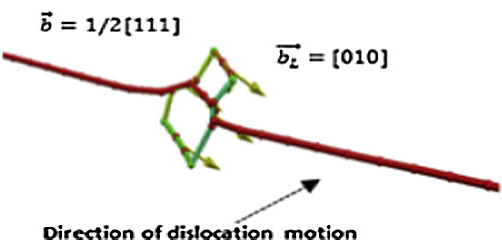
\includegraphics[height=0.15\textheight]{img/comparaison-xshi-dd}
		\caption{Dynamique des Dislocations.}
	\end{subfigure}
	\caption[Comparaisons DD / MD]{Comparaison entre les résultats de Dynamique Moléculaire et de Dynamique des dislocations \citebiblio{shi2015comparaison}.}
	\label{fig:comparaison_md}
\end{figure}
%interaction of <100> dislocation loops with dislocations studied by dislocation dynamics in alpha iron - XJ Shi

Des travaux récents permettent d'extraire les lignes de dislocation des simulations de Dynamique Moléculaire \citebiblio{ovitowassim}, ce qui permettra de comparer plus finement les résultats des deux méthodes.

\subsubsection{Résultats déduits par la DDD}
\label{sec:resultats ddd}

Les simulations de dynamique des dislocations permettent de mieux comprendre la formation de jonctions et leur lien avec l'écrouissage \citebiblio{bulatov2006nature}. La visualisation des résultats de simulation permettent des observations phénoménologiques difficilement visibles expérimentalement.

La Dynamique des Dislocations permet aussi d'affiner le modèle de Taylor pour les phénomènes d'écrouissage \citebiblio{devincre2006physical}. La simulation permet de contrôler la distribution initiale des dislocations plus facilement que dans des conditions réelles. Cela permet, par exemple, de sélectionner un système de glissement afin d'étudier des propriétés comme sa contrainte d'activation.

%http://iopscience.iop.org/article/10.1088/0965-0393/15/6/001/meta
%devincre - coef taylor - http://www.sciencedirect.com/science/article/pii/S1359646205007128
%durcissement taylor - http://www.sciencedirect.com/science/article/pii/0001616080901625

Les effets de l'irradiation sur les matériaux peuvent être quantifiés par la Dynamique des dislocations. L'étude des interactions entre les dislocations et les boucles d'irradiations permettent de mieux comprendre les phénomènes de durcissement par irradiation \citebiblio{shi2014these}. L'étude de la formation de bandes claires \citebiblio{nogaret2008} permettent de mieux comprendre la fragilisation sous irradiation.

\end{document}